% Make nice A4 pages for print:
%\usepackage{pgfpages}
%\pgfpagesuselayout{resize to}[a4paper,border shrink=5mm,landscape]

\beamertemplatenavigationsymbolsempty

\setbeamertemplate{bibliography item}[text]

\usepackage[type={CC},modifier={by-sa},version={4.0}]{doclicense}

\usepackage[utf8]{inputenc}
\usepackage{hyperref}
\usepackage{breakurl}
\usepackage{graphicx}
\usepackage{pgfplots}
\usepackage{pgf}
\usepackage{tikz}
\usetikzlibrary{positioning}
\usetikzlibrary{arrows}
\usetikzlibrary{decorations.markings}
\usetikzlibrary{calc}
\usetikzlibrary{matrix}
\usetikzlibrary{shapes}
\usetikzlibrary{decorations.pathmorphing}
\usetikzlibrary{fit}
\usetikzlibrary{backgrounds}
\usetikzlibrary{plotmarks}
\usepackage{stmaryrd}
\usepackage{listings}
\usepackage{pdflscape}
\usepackage{perpage}
\usepackage{appendixnumberbeamer}

%\usepackage[thmmarks,amsmath,amsthm]{ntheorem} % already included in beamer
\usepackage{thm-restate}

\usepackage[sort&compress,numbers]{natbib}  % to be have \citet, \citeauthor, \citeyear

\MakePerPage{footnote}

\tikzstyle{o}=[r,ppBlue]
\tikzstyle{r}=[thick,rectangle,align=center]
\tikzstyle{t}=[r,ppTrans] %,font=\bfseries]
\tikzstyle{dd}=[densely dashed]
\tikzstyle{n}=[r,ppBlue]
\tikzstyle{p}=[r,ppRed]
\tikzstyle{ppRed}  =[draw=red,  fill=  red!20]
\tikzstyle{ppBlue} =[draw=blue, fill= blue!20]
\tikzstyle{ppGreen}=[draw=green,fill=green!20]
\tikzstyle{ppTrans}=[draw=none, fill=none]

\usetheme{Warsaw}

\useoutertheme[subsection=true]{smoothbars}
%\useoutertheme[subsection=false]{miniframes}

\definecolor{bblue}{HTML}{D7DF01}	% yellow-ish actually, for better black/white printing
\definecolor{rred}{HTML}{C0504D}
\definecolor{ggreen}{HTML}{9BBB59}
\definecolor{ppurple}{HTML}{9F4C7C}
\definecolor{lightgray}{rgb}{0.3,0.3,0.3}
\definecolor{lightergray}{rgb}{0.9,0.9,0.9}
\definecolor{UniBlue}{RGB}{83,121,170}

\DeclareTextFontCommand\textintro{\normalfont\bfseries\itshape} % nice!
\newcommand{\intro}[2][]
{%
	\textintro{#2}%
}
\newcommand{\empha}[2][]
{%
	\emph{#2}%
}

%\theoremstyle{plain}
\newcounter{reqcounter}
\newtheorem{requirement}[reqcounter]{Requirement}

%setbeamercolor{structure}{fg=violet}

\makeatletter
\def\th@task{%
    \normalfont % body font
    \setbeamercolor{block title example}{bg=orange,fg=white}
    \setbeamercolor{block body example}{bg=orange!20,fg=black}
    \def\inserttheoremblockenv{exampleblock}
  }
\makeatother

\theoremstyle{task}
\newtheorem{task}{Task}

\newenvironment{assignment}%
{%\setbeamercolor{background canvas}{bg=violet}%
%\setbeamercolor{structure}{fg=cyan!90!black}%
 \setbeamercolor{frametitle}{bg=orange,fg=white}
\begin{frame}}%
{\end{frame}}%

\AtBeginSection[]{
  \begin{frame}
  \vfill
  \centering
  \begin{beamercolorbox}[sep=8pt,center,shadow=true,rounded=true]{title}
    \usebeamerfont{title}\insertsectionhead\par%
  \end{beamercolorbox}
  \tableofcontents
  \vfill
  \end{frame}
}




\pgfplotsset{compat=1.14}
\author{Markus Raab}


\title{L10 Design of Configuration}
\date{16.06.2021}

\begin{document}




%%%%%%%%%%%%%%%%%%%%%%%%%%%%%%%%%%%%%%%%%% 
\section{Documentation}

\begin{frame}
	\frametitle{Learning Outcomes}
	Students will be able to

	\begin{itemize}
	\item remember connections between the many different topics within CM
	\item design and document configuration settings and specifications
	\item evaluate a configuration system and decide about use of
	\begin{itemize}
	\item code generation
	\item introspection
	\end{itemize}
	\end{itemize}
\end{frame}

\begin{frame}[fragile]
	\frametitle{Three Places}

	There are at least three places where documentation can be.

	\begin{enumerate}
	\item In the CM code.
	\item In the specification (e.g., metadata ``description''):
	\begin{code}[gobble=4]
	[slapd/threads/listener]
	  description:=adjust to use more threads
	\end{code}
	\item In comments of config files (e.g., metadata ``comment'').
	\end{enumerate}

	We will mostly talk about documentation of the specification.
\end{frame}


\begin{frame}
	\ExecuteMetaData[../book/motivation.tex]{documentation-inform}
\end{frame}

\begin{frame}
	There are at least two forms of documentation necessary:

	\begin{itemize}
	\item Explanations
	\item Examples
	\end{itemize}

	Generation helps to avoid duplication:

	\ExecuteMetaData[../book/motivation.tex]{documentation-req}
\end{frame}

\begin{frame}
	\begin{alertblock}{Question}
	How to avoid duplication between description text and other parts?
	\end{alertblock}

	\pause

	\begin{itemize}
	\item Render type and defaults into the documentation
	\item Render requirements and rationale into the documentation
	\item Render any other semantics into the documentation
	\end{itemize}
\end{frame}

\begin{frame}[fragile]
	\frametitle{Example}

	\begin{code}[gobble=4]
	[slapd/threads/listener]
	  check/range:=1,2,4,8,16
	  default:=1
	  description:=adjust to use more threads
	  rationale:=needed for many-core systems
	  requirement:=1234
	  visibility:=user
	\end{code}
\end{frame}

\begin{frame}[fragile]
	\frametitle{Semantics}

	Avoid describing semantics that easily can be specified:

	\begin{code}[gobble=4]
	[app/log/file]
	  description:=path to file for logs
	\end{code}

	Instead use:

	\begin{code}[gobble=4]
	[app/log/file]
	  check/path:=
	\end{code}
\end{frame}

\begin{frame}
	\frametitle{Reevaluate specifications}

	In which situations should you reevaluate if a configuration setting (specification) is needed?

	\ExecuteMetaData[../book/implications.tex]{reasons-adding}
\end{frame}

\begin{frame}
	\frametitle{Design Decisions}

	There are many ways to design configuration access but many decisions are only pragmatic and irrelevant with proper key/value abstraction.

	\begin{task}
	Which design decisions are there?
	Why are they (ir)relevant?
	\end{task}

	\pause

	\begin{itemize}
	\item Which configuration file format? (irrelevant due to key/values)
	\item Split up into multiple configuration files? (irrelevant due to 3-way merging)
	\item Where are the configuration files? (irrelevant due to mounting and resolver)
	\item Important: Introspection, Validation, Modularity, Specifications, API, Guarantees, Docu \dots
	\end{itemize}
\end{frame}






%%%%%%%%%%%%%%%%%%%%%%%%%%%%%%%%%%%%%%%%%% 
\section{Introspection}

\subsection{}

\begin{frame}
	\frametitle{Introspection}
	\begin{alertblock}{Question}
	What can introspection offer?
	\end{alertblock}

	\pause
	\begin{itemize}
	\item unified get/set access to (meta*)-key/values
	\item GUI, web-UI can semantically interpret metadata
	\item access via applications, CLI, GUI, web-UI, ...
	\item access via any programming language (similar to file systems)
	\item access via any configuration management system
	\end{itemize}
\end{frame}

\begin{frame}[fragile]
	\frametitle{Internal Specification}

	For example, OWNER:
	\begin{code}[gobble=4,language=Java]
	import org.aeonbits.owner.Config;

	public interface ServerConfig extends Config {
		int port();
		String hostname();
		@DefaultValue("42")
		int maxThreads();
	}
	\end{code}
\end{frame}

\begin{frame}
	\begin{alertblock}{Question}
	Why do we need an external specification?
	\end{alertblock}

	\pause
	\vspace{1em}

	\textbf{Introspection}:
	\begin{itemize}
	\item needed as communication of producers and consumers of configuration
	\item the foundation for any advanced tooling like configuration management tools
	\item essential for \intro[no-futz computing]{no-futz computing}~\citet{holland2001nofutz}
	\end{itemize}
\end{frame}

\begin{frame}[fragile]
	\frametitle{External Specification}

	\begin{code}[gobble=4]
	[port]
	type:=long
	[hostname]
	default:=42
	[threads/max]
	type:=long
	\end{code}

	\vspace{1em}

	Advantages:
	\pause
	\begin{itemize}
	\item are read and writable by other applications (introspection)
	\item we can generate the internal specification (code generation)
	\item we fulfill needs for configuration management tools
	\end{itemize}
\end{frame}

\begin{frame}
	Other artefacts:

	\pause

	\begin{itemize}
	\item examples (e.g., defaults)
	\item documentation
	\item auto-completion/syntax highlighting/IDE support
	\item tooling (GUI, Web UI)
	\item validation code
	\item parsing code (e.g., command-line parsing)
	\item CM code
	\item configuration access APIs
	\end{itemize}
\end{frame}

\begin{frame}
	\frametitle{KeySet (Recapitulation)}

	The common data structure between plugins:
	\vspace{1cm}

	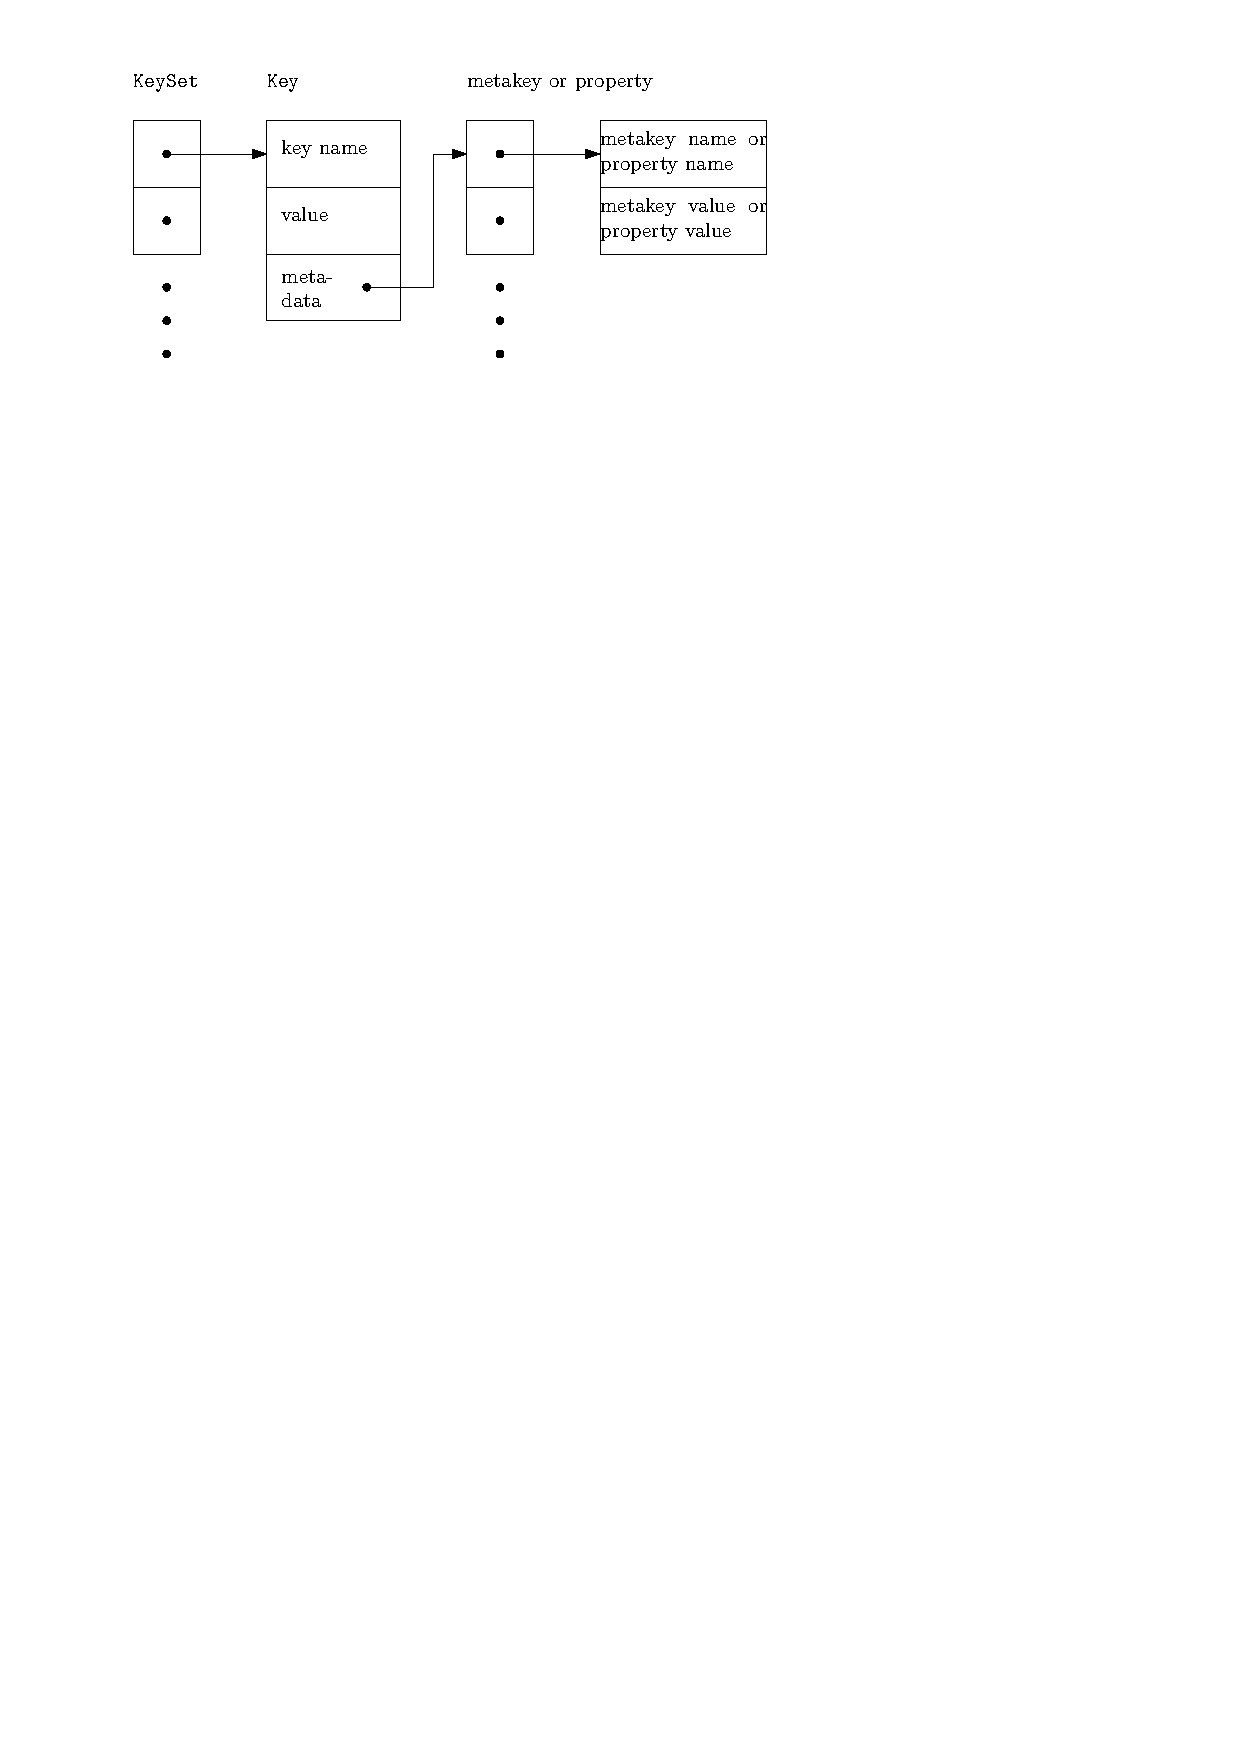
\includegraphics{keyset}
\end{frame}

\begin{frame}[fragile]
	\frametitle{KeySet Generation}
	\begin{alertblock}{Question}
	Idea: What if the configuration file format grammar describes source code?
	\end{alertblock}

	\pause

	key ^spec:/slapd/threads/listener^, with the configuration value ^4^ and the property $\property{default} \mapsto 1$:

	\begin{code}[gobble=4,language=Cpp]
	ksNew (keyNew ("spec:/slapd/threads/listener",
		       KEY_VALUE, "4",
		       KEY_META, "default", "1",
		       KEY_END),
	       KS_END);
	\end{code}

	\begin{alertblock}{Finding}
	We get source code representing the settings.
	\end{alertblock}
\end{frame}

\begin{frame}
	\frametitle{Possible Properties (Recapitulation)}

	For example, SpecElektra has following properties:
	\begin{description}
	\item[type] represents the type to be used in the emitted source code.
	\item[opt] is used for short command-line options to be copied to the namespace \namespace{proc}.
	\item[opt/long] is used for long command-line options, which differ from short command-line options by supporting strings and not only characters.
	\item[default] enables us to start the application even if the backend does not work.
	\end{description}
\end{frame}

\begin{frame}
	\frametitle{Introspection vs. Code Generation}

	\setbeamersize{description width=1cm}
	\begin{description}
	\item[$-$] more techniques for performance improvements with code generation
	\item[$+$] specification can be updated live on the system without recompilation
	\item[$+$] tooling has generic access to all specifications
 	\item[$+$] new features the key database (e.g., better validation) are immediately available consistently
	\end{description}

	\vspace{0.5em}

	\begin{alertblock}{Implication}
	We generally prefer introspection, except for a very thin configuration access API.
	\end{alertblock}
\end{frame}



%%%%%%%%%%%%%%%%%%%%%%%%%%%%%%%%%%%%%%%%%% 
\section{Code Generation}

\subsection{Why?}

\begin{assignment}
	\begin{task}
	How to ensure that configuration access points match with present configuration settings?
	\end{task}
\end{assignment}

\begin{frame}
	\frametitle{Rationale (Partly Recapitulation)}
	Configuration Specification:
	\begin{itemize}
	\item without specification you and others do not even know which settings are available
	\item needed for any further techniques we will discuss:
		\begin{itemize}
		\color{red}
		\item code generation guarantees that configuration access points match with specification
		\item validation guarantees that configuration settings match with specification
		\end{itemize}
	\item essential for \intro[no-futz computing]{no-futz computing}~\citet{holland2001nofutz}
	\item the foundation for any advanced tooling like configuration management tools
	\item needed as communication of producers and consumers of configuration
	\end{itemize}
\end{frame}

\begin{frame}[fragile]
	\frametitle{Current Challenges}
	Configuration access code usually has:
	\pause
	\begin{itemize}
	\item code duplications and unsafe APIs
	\item hard-coded default values
	\item unexpected transformations (e.g., truncating of values)
	\item inconsistencies (e.g., case sensitivity)
	\item no introspection facilities (which keys and values are allowed?)
	\end{itemize}
	\begin{example}[Silent Overruling \cite{xu2013blame}]
	\begin{code}[gobble=4,language=C++]
	if (!strcasecmp(token, "on")) {
		*var = 1;
	} else {
		*var = 0;
	} /* src/cache_cf.cc from Squid */
	\end{code}\end{example}
\end{frame}

\begin{frame}[fragile]
	\frametitle{Real-world example}
	PostgreSQL\footnote{\url{http://doxygen.postgresql.org/guc_8c_source.html}} has following duplications for its configuration settings:
	\begin{itemize}
	\item a global variable and an option record (struct)
	\item an entry in an example (postgresql.conf.sample)
	\item documentation in sgml
	\item in the source code of utils (in-source dump utils, and dozens of external configuration management tools)
	\end{itemize}
	\pause
	\vspace{1em}
	Note: PostgreSQL has a clean implementation, and above list only shows limitations of systems without code generation.
\end{frame}

\begin{assignment}
	\begin{task}
	Brainstorming: Which artefacts can we produce with (code) generation?
	\end{task}
\end{assignment}

\begin{frame}
	Artefacts:
	\begin{itemize}
	\item examples (e.g., defaults)
	\item documentation
	\item auto-completion/syntax highlighting/IDE support
	\item tooling (GUI, Web UI)
	\item validation code
	\item CM code
	\item configuration access APIs
	\end{itemize}
\end{frame}

\begin{frame}
	\frametitle{Goal}

	\begin{goal}
	Configuration settings should adhere the specification from source to destination.
	\end{goal}

	\begin{restatable}{requirement}{reqGeneration}
	The specification must enable code generation and inconsistencies must be ruled out during compilation.
	\end{restatable}
\end{frame}


\subsection{How?}

\begin{frame}
	\frametitle{Code Generation}

	\ExecuteMetaData[../book/approach.tex]{code-generation}

	\pause
	\vspace{2em}
	But how?
\end{frame}

\begin{frame}
	\frametitle{KeySet (Recapitulation)}

	The common data structure between plugins:
	\vspace{1cm}

	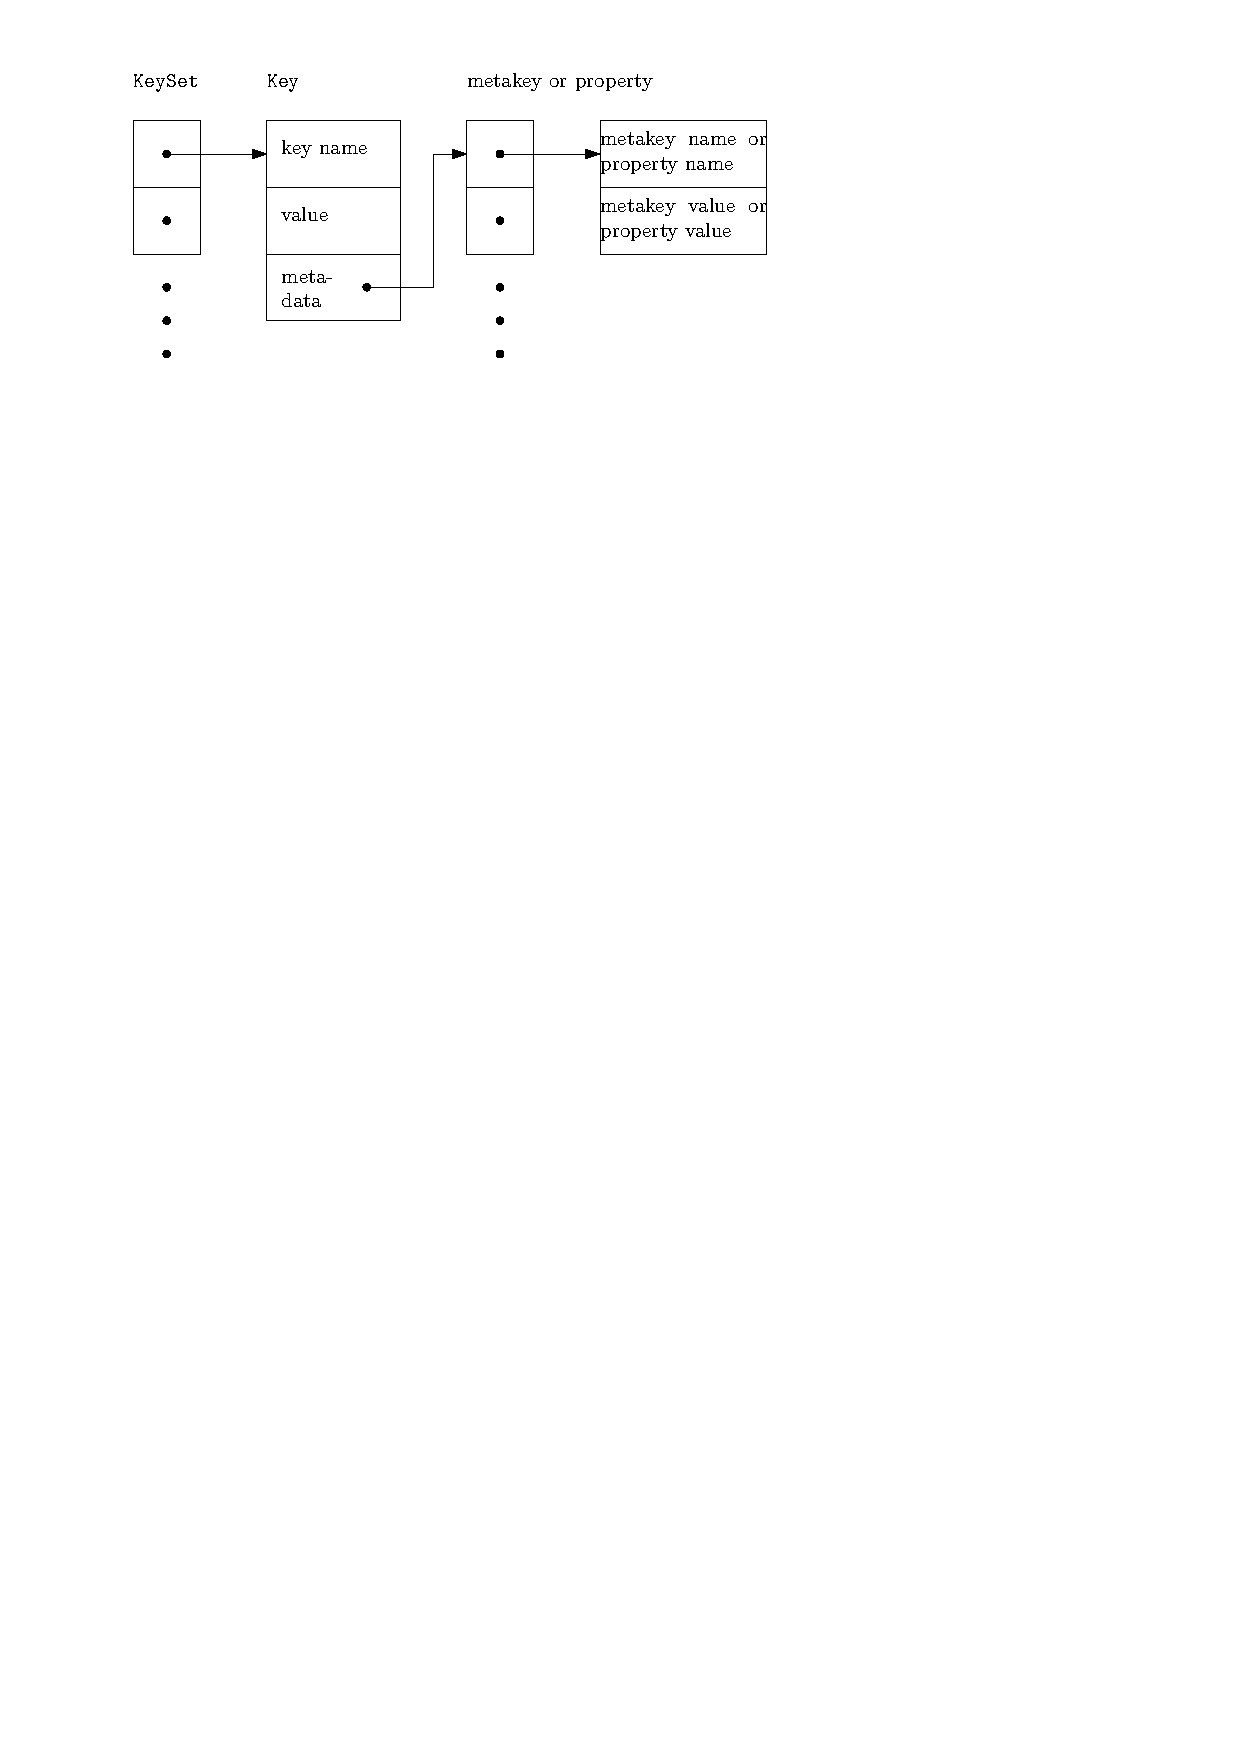
\includegraphics{keyset}
\end{frame}

\begin{frame}[fragile]
	\frametitle{KeySet Generation}
	\begin{alertblock}{Question}
	Idea: What if the configuration file format grammar describes source code?
	\end{alertblock}
	\pause

	\begin{grammar}
	<KeySet> ::= \lq ksNew'\WhiteSpace(' \{ <Key> \lq , \LineBreak'  \}  \{ \lq\WhiteSpace' \} \lq KS\_END);'

	<Key> ::= \lq keyNew \WhiteSpace ('' ' <key name> \lq ''  , \LineBreak' [ <Value> ] <properties> \lq KEY_END)'

	<Value> ::=  \{ \lq\WhiteSpace' \} \lq KEY\_VALUE, \WhiteSpace '' ' <configuration value> \lq ''  , \LineBreak'

	<properties> ::= \{ \{ \lq\WhiteSpace' \} <property> \lq , \LineBreak' \}

	<property> ::=  \lq KEY\_META, \WhiteSpace " ' <property name> \lq "  , \WhiteSpace " ' <property value> \lq " '
	\end{grammar}
\end{frame}

\begin{assignment}
	\begin{task}
	Break.
	\end{task}
\end{assignment}

\begin{frame}[fragile]
	\frametitle{Example}
	\begin{example}
	Given the key ^spec:/slapd/threads/listener^, with the configuration value ^4^ and the property $\property{default} \mapsto 1$, \elektra{Gen} emits:

	\begin{code}[gobble=4,language=Cpp]
	ksNew (keyNew ("spec:/slapd/threads/listener",
		       KEY_VALUE, "4",
		       KEY_META, "default", "1",
		       KEY_END),
	       KS_END);
	\end{code}
	\vspace{-1em}
	\end{example}

	\pause
	\begin{alertblock}{Finding}
	We have source code representing the settings.
	And if we instantiate it, we have a data structure representing the settings.
	Plugins emitting such ``configuration files'' are code generators.
	\end{alertblock}
\end{frame}

\begin{frame}[fragile]
	\frametitle{Implementation Strategies}

	\begin{itemize}
	\item Using ^print^ (only for very small generators)
	\item Using generative grammars
	\begin{code}[gobble=4,language=Cpp]
	query = '{' >> *(pair) > '}';
	pair = '{' >> key_name > '=' >> key_value >>
	       *('{' >> metakey_name > '=' >> metakey_value > '}')
	       > '}';
	\end{code}
	\item Using template languages (RubyERB, Cheetah, Mustache)
	\begin{code}[gobble=4,language=Python,basicstyle=\ttfamily\tiny,numberstyle=\ttfamily\tiny\color{blue}]
	@for n in hierarchy.name.split('/')[1:-1]
	namespace $support.nsnpretty($n)
	{
	class ${hierarchy.prettyclassname(support)}
	{
	typedef $support.typeof($hierarchy.info) type;
	@if $support.typeof($hierarchy.info) != "kdb::none_t"
	static type get(kdb::KeySet &ks, kdb::Key const& spec)
	{
		type value $support.valof($hierarchy.info)
		Key found(ckdb::ksLookup(ks.getKeySet(), *spec,
					ckdb::elektraLookupOptions::KDB_O_SPEC));
		return found.get<$support.typeof($hierarchy.info)>();
	}
	\end{code}
	\end{itemize}
\end{frame}

\begin{frame}
	\frametitle{Possible Properties}
	For example, SpecElektra has following properties:
	\begin{description}
	\item[type] represents the type to be used in the emitted source code.
	\item[opt] is used for short command-line options to be copied to the namespace \namespace{proc}.
	\item[opt/long] is used for long command-line options, which differ from short command-line options by supporting strings and not only characters.
	\item[restrict/write] yields compilation errors when developers assign a value to a contextual value within the program.
	\item[default] enables us to start the application even if the backend does not work.
	\end{description}
\end{frame}

\begin{frame}[fragile]
	With the specification:
	\par
	\begin{code}[gobble=4]
	[foo/bar]
	  default:=Hello
	  type:=string
	  opt:=b
	  restrict/write:=1
	\end{code}
	\par
	\elektra{Gen} gives the user read-only access to the object ^env.foo.bar^:
	\par
	\begin{code}[language=Cpp]
	std::cout << env.foo.bar;
	env.foo.bar = "Other world"; // comp. error
	\end{code}
	\par
	\small
	\pause
	Line~1 prints the configuration value of ^/foo/bar^ or ^"Hello"^ (without quotes) by default.
	When invoking the application with ^application -b "This world"^, the application would print ^"This world"^ (without quotes).
	Line~2 leads to a compilation error because of the property \property{restrict/write}.
\end{frame}

\begin{frame}[fragile]
	\frametitle{Which Configuration Access API?}

	First approach, one class (or function) per configuration setting:
	\\[1em]
	\begin{code}[gobble=4,language=Cpp]
	class SlapdThreadsListener : public Value<long,
		WritePolicyIs<ReadOnlyPolicy>> {
		... keyNew ("/slapd/threads/listener",
			    KEY_META, "type", "long",
			    KEY_META, "restrict/write", "1",
			    KEY_END) ...
	};
	\end{code}
\end{frame}

\begin{frame}[fragile]
	\frametitle{Which Configuration Access API?}

	Bad idea, manual instantiation and long names necessary:
	\\[1em]
	\begin{code}[gobble=4,language=Cpp]
	KeySet config;
	Context c;
	long foo ()
	{
		SlapdThreadsListener slapdThreadsListener (config, c);
		slapdThreadsListener++;
		return slapdThreadsListener;
	}
	\end{code}
\end{frame}

\begin{frame}[fragile]
	\frametitle{Which Configuration Access API?}

	Use hierarchy with namespaces or nested classes:
	\\[1em]
	\begin{code}[gobble=4,language=Cpp]
	namespace slapd
	{
	namespace threads
	{
	class Listener : public Value<long> {};
	}  // <continues on the next page>
	class Threads : public Value<none_t>
	{threads::Listener listener;};
	}  // end namespace slapd
	class Slapd : public Value<none_t>
	{slapd::Threads threads;};
	class Environment {Slapd slapd;};
	\end{code}
\end{frame}

\begin{frame}[fragile]
	\frametitle{Which Configuration Access API?}

	Much easier to use:
	\begin{code}[gobble=4,language=Cpp]
	long foo(slapd::Threads const & threads)
	{
		threads.listener++;
		Context & c = threads.context ();
		return threads.listener;
	}

	int main()
	{
		KeySet config;
		Context c;
		Environment env (config, c);
		long x = foo (env.slapd.threads);
	}
	\end{code}
\end{frame}

\begin{frame}[fragile]
	\frametitle{Which Configuration Access API?}

	In C, we use identifiers to be passed to the highlevel API\footnote{\url{https://www.libelektra.org/tutorials/high-level-api}}:
	\\[2em]
	\begin{code}[gobble=4,language=Cpp]
	elektraGetString (elektra, ELEKTRA_TAG_MY);
	\end{code}
	Where ^ELEKTRA_TAG_MY^ is a struct for that type.
	\\[2em]

	We can also omit the type:
	\begin{code}[gobble=4,language=Cpp]
	elektraGetLong (elektra, ELEKTRA_TAG_THREADS);
	elektraGet (elektra, ELEKTRA_TAG_THREADS);
	\end{code}
\end{frame}

\begin{frame}
	Guarantees by code generation:
	\begin{itemize}
	\item Every configuration setting is specified (essential for refactoring).
	\item (Data) type of source code and configuration settings match.
	\item Configuration access with defaults is always successful.
	Reason: We use defaults if everything else fails.
	\end{itemize}
	\vspace{3em}
	Missing Guarantee: Is every specified setting actually used?
\end{frame}



%%%%%%%%%%%%%%%%%%%%%%%%%%%%%%%%%%%%%%%%%% 
\section{Introspection vs. Generation}

\subsection{}

\begin{frame}
	\begin{alertblock}{Question}
	Introspection vs. Code Generation?
	\end{alertblock}
\end{frame}

\begin{frame}
	Limitations of introspection:
	\begin{itemize}
	\item no static checks
	\item no whole-program optimizations (API barriers)
	\end{itemize}
\end{frame}

\begin{frame}
	Overhead without code generation (=backend) is $1.8$x higher~\cite{raab2015kps}:
	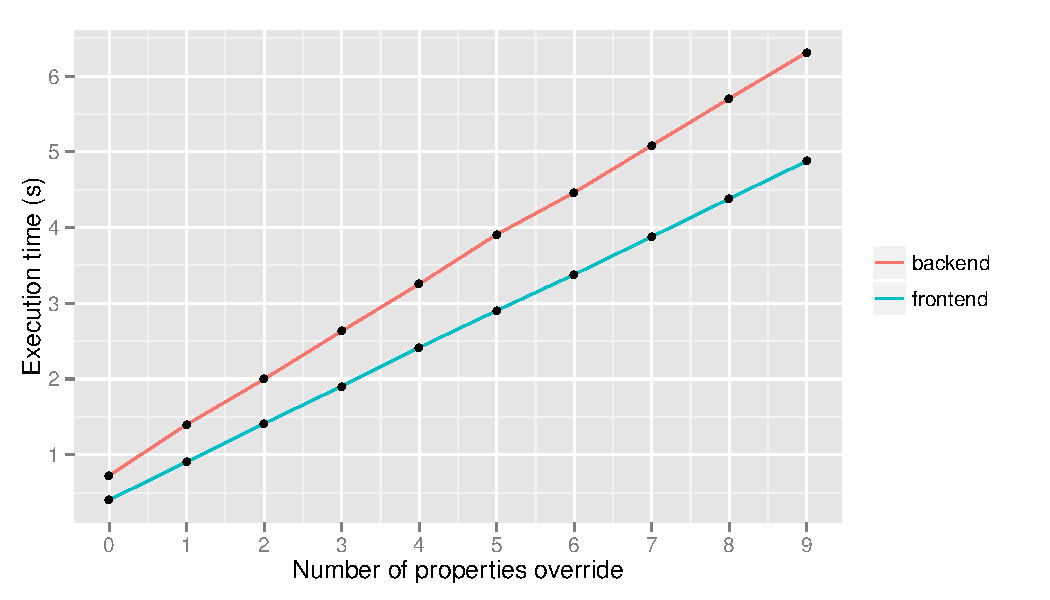
\includegraphics[width=\textwidth]{mean2}
\end{frame}

\begin{frame}
	But it might not matter because configuration access might not be a bottleneck~\cite{raab2015kps},
	for example, a word counting application:

	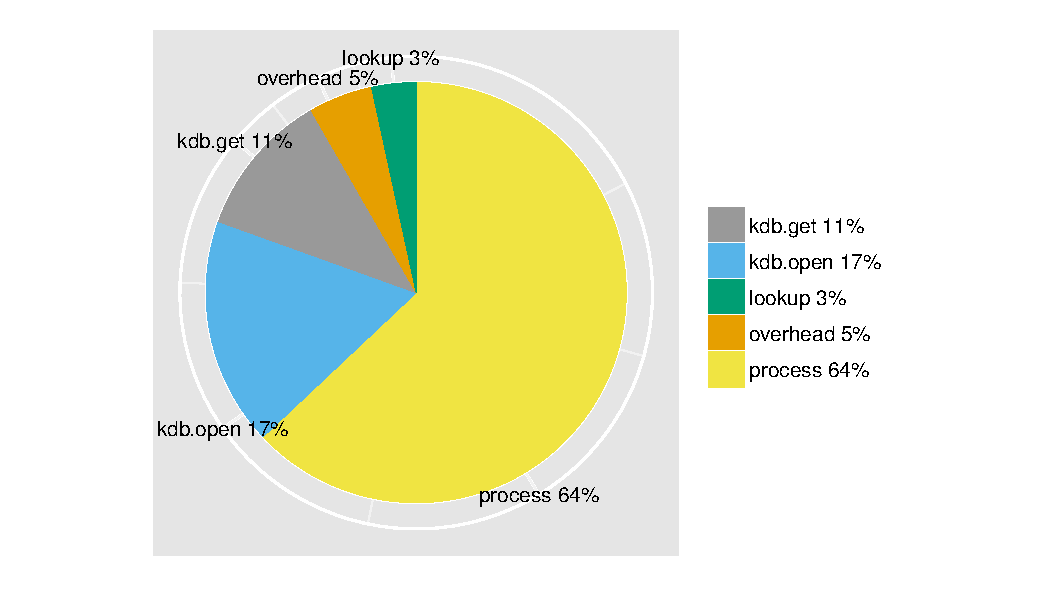
\includegraphics[width=\textwidth]{wc}

	But: \pause
	Configuration access points within loops might be a bottleneck.
\end{frame}

\begin{frame}
	Advantages of introspection:
	\pause
	\begin{itemize}
	\item specification can be updated live on the system without recompilation
	\item tooling has generic access to all specifications
 	\item new features the key database (e.g., better validation) are immediately available consistently
	\end{itemize}
	\vspace{1em}
	\begin{alertblock}{Implication}
	We generally prefer introspection, except for a very thin configuration access API.
	\end{alertblock}
	\vspace{1em}
	\begin{restatable}{requirement}{reqIntrospection}
	Configuration settings and specifications must be introspectable.%
	\end{restatable}
\end{frame}

\begin{frame}
	\frametitle{Use Cases of Elektra}
	\begin{itemize}[<+->]
	\item Embedded systems
	\begin{itemize}
	\item OpenWRT (distribution)
	\item Broadcom (blue-ray devices)
	\item Kapsch (cameras)
	\item Toshiba (TVs)
	\end{itemize}
	\item Server
	\begin{itemize}
	\item Allianz (insurance)
	\item TU Wien
	\item puppet-libelektra
	\item Other Universities
	\end{itemize}
	\item Desktop
	\begin{itemize}
	\item Oyranos
	\item LCDproc (in progress)
	\item KDE
	\end{itemize}
	\end{itemize}
\end{frame}

\begin{frame}
	\frametitle{Conclusion}
	\begin{itemize}
	\item goals:
		\begin{itemize}
		\item make simple configuration management tasks simple
		\item improve robustness
		\item improve extensibility (reusable plugins operating on key/value)
		\item improve performance
		\item good defaults
		\item system-wide introspection
		\item system-level dependency injection
		\end{itemize}
	\item \elektra{} has no dependence to other libraries but only concrete plugins introduce dependences.
	\end{itemize}
\end{frame}




%%%%%%%%%%%%%%%%%%%%%%%%%%%%%%%%%%%%%%%%%% 
\section{Context-Awareness}

\subsection{}

\begin{frame}
	\citet{khalil2005context} conducted a study where all users found context-aware configuration (very) useful.
	They learned that in \p{89} of cases the mapping between activities and settings was consistent for individual users.
	In the study, context-aware configuration improved satisfaction, even if deduced settings sometimes were not appropriate.
	For example, a participant stated:
	\vspace{2em}

	\begin{quote}
	``I like how it changes state without you having to tell it to. I always forget to turn my cell [off] in class and turn it on after.''
	\end{quote}
\end{frame}

\begin{frame}
	\frametitle{Definition (Recapitulation)}
	\ExecuteMetaData[../book/background.tex]{context-definition}
\end{frame}

\begin{frame}
	\frametitle{Types of Configuration (Recapitulation)}
	\pause
	\begin{description}
	\ExecuteMetaData[../book/background.tex]{context-types}
	\end{description}
\end{frame}

\begin{frame}
	\frametitle{Cascading (Recapitulation)}
	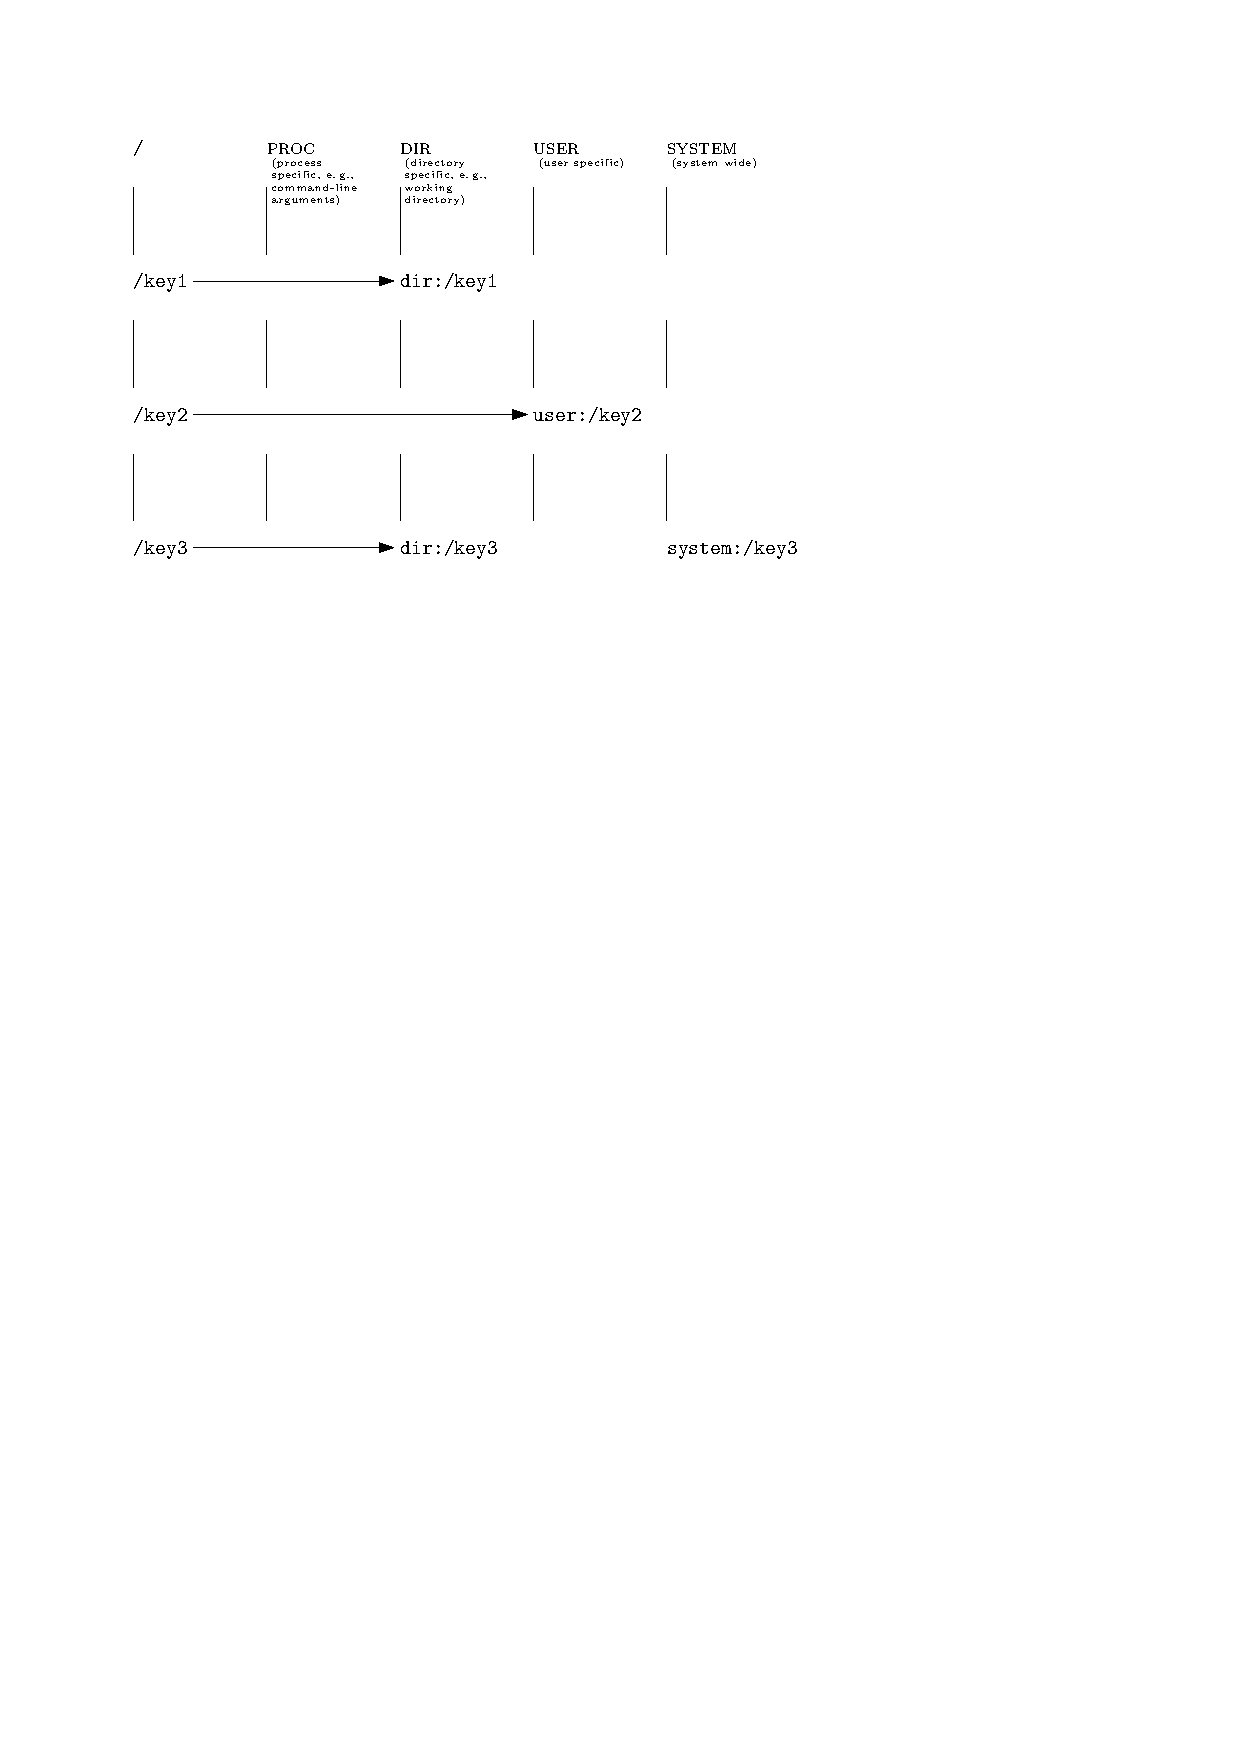
\includegraphics{cascading}
\end{frame}

\begin{frame}
	\frametitle{Context-oriented Programming}
	\ExecuteMetaData[../book/background.tex]{context-oriented-programming}
\end{frame}

\begin{frame}
	\frametitle{Contextual Values}
	\ExecuteMetaData[../book/background.tex]{contextual-values}
\end{frame}

\begin{frame}[fragile]
	\frametitle{Contextual Values (Pseudocode)}

	\begin{code}[gobble=4,language=C++,morekeywords={context}]
	void printBrowserConfig (Config config)
	{
		context.with("private")
		{
			println (config.keepHistory);
		}
		// same thread, different context:
		println (config.keepHistory);

		context.activate(currentLocation)
	}
	\end{code}
\end{frame}
\begin{frame}
	\frametitle{Introspection vs. Code Generation (Partly Recapitulation)}

	Implementation of contextual values might be in key database or in generated code.
	Advantages of having it in key database (with introspection)?

	\pause

	\setbeamersize{description width=1cm}
	\begin{description} %[leftmargin=0cm] %TODO: move left
	\item[$-$] more techniques for performance improvements with code generation
	\item[$+$] specification can be updated live on the system without recompilation
	\item[$+$] tooling has generic access to all specifications
 	\item[$+$] new features the key database (e.g., better validation) are immediately available consistently
	\item[$-$] \color{red} needed if context differs within same thread
	\end{description}

	\vspace{0.5em}

	\begin{alertblock}{Implication}
	We generally prefer introspection, except for a very thin configuration access API.
	\end{alertblock}
\end{frame}


\begin{assignment}
	\begin{task}
	Break.
	\end{task}
\end{assignment}

\begin{frame}
	\frametitle{Types of Specifications (Recapitulation)}
	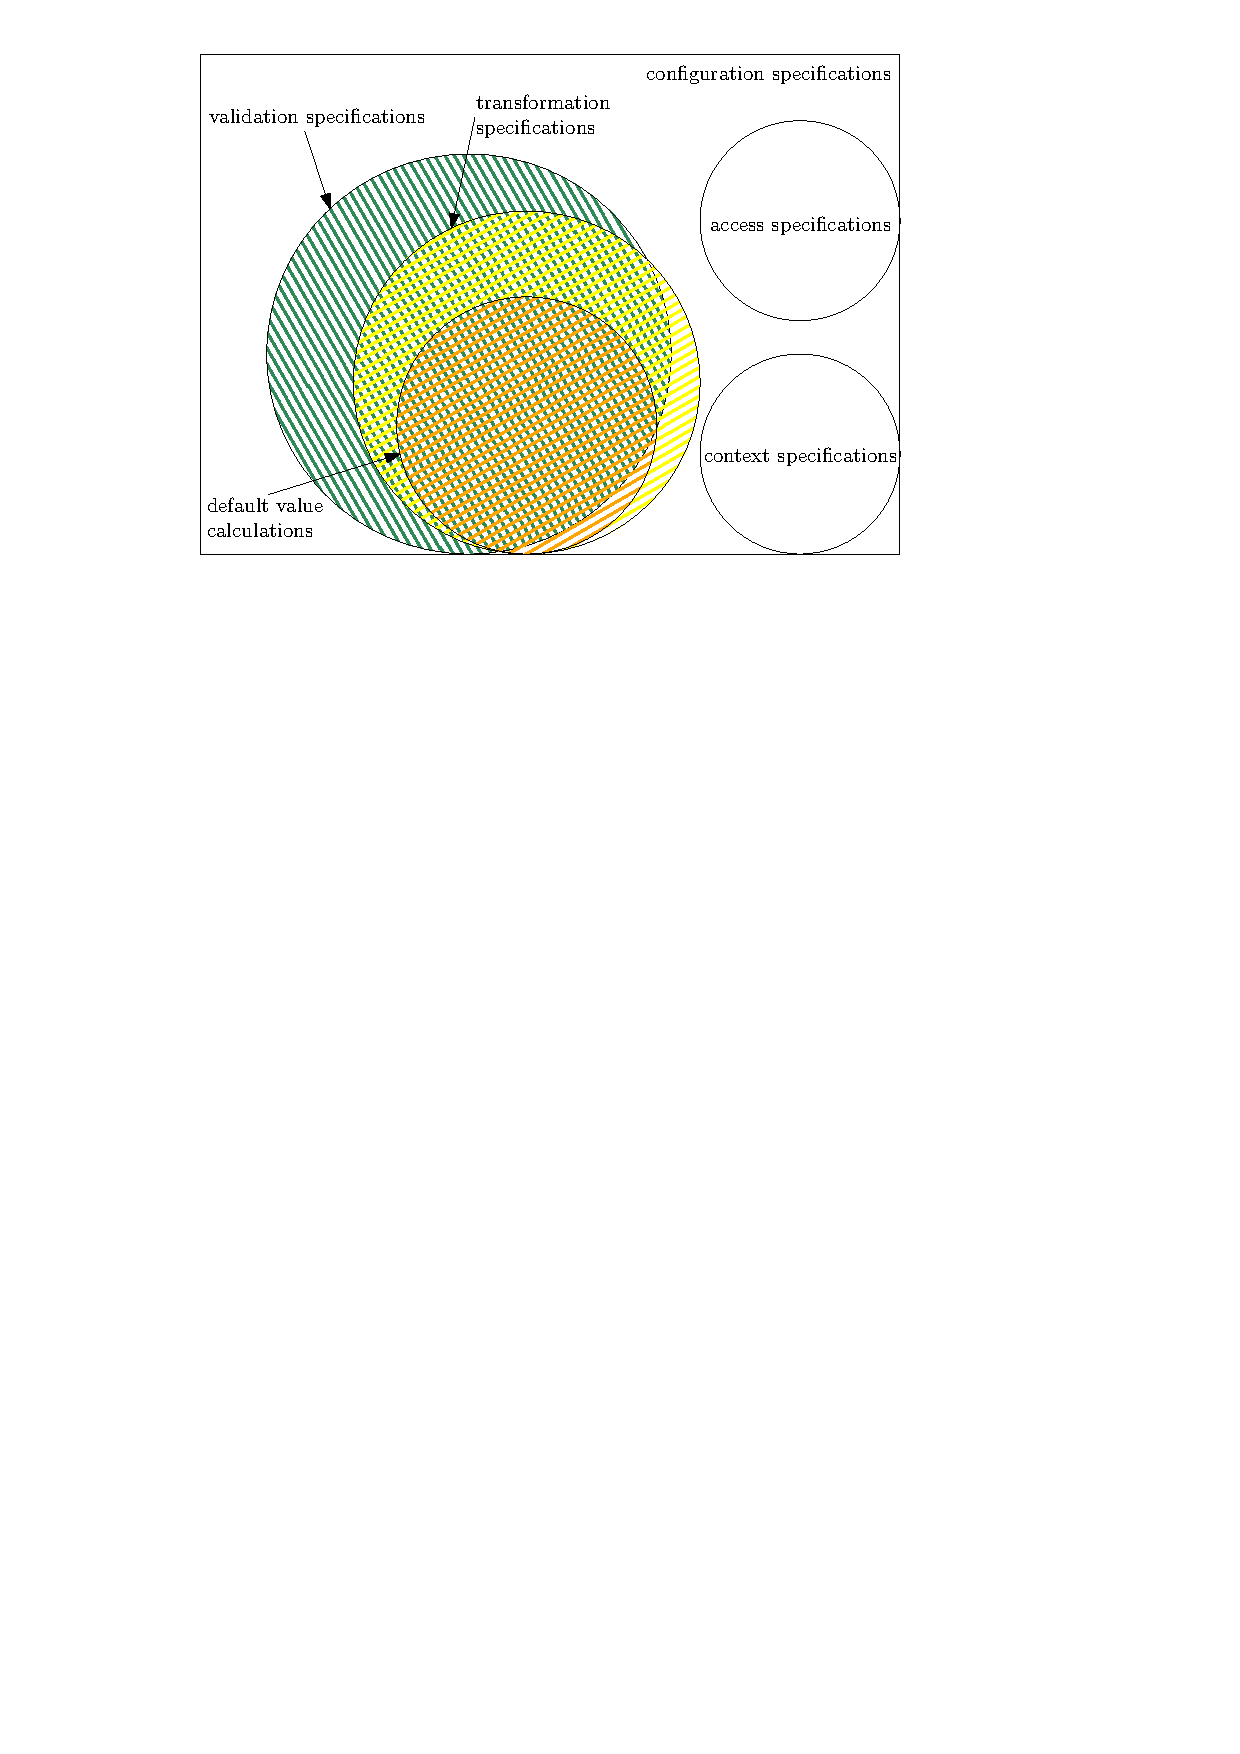
\includegraphics[scale=0.8]{specifications}
\end{frame}

\begin{frame}
	\frametitle{Keys as Contextual Values}

	\begin{itemize}[<+-| alert@+>]
	\item keys can be interpreted as contextual values~\cite{raab2016persistent,raab2017introducing}
	\item we can make contextual values dependent on contextual values
	\item we can also use keys to describe requirements
	\item if we use a predefined path in Elektra for layers, we can activate context by writing to KDB
	\item this is implemented in ``kdb elektrify-getenv''
	\end{itemize}

	\pause[\thebeamerpauses]

	\begin{alertblock}{Implication}
	The configuration can fully describe the context and the requirements.
	\end{alertblock}
\end{frame}

\begin{frame}[fragile]
	\frametitle{Context Specifications}

	\begin{itemize}
	\item
	Determine threads from CPUs:

	\begin{code}[gobble=4]
	[env/layer/cpu]
	  type:=long
	[slapd/threads/listener]
	  context:=/slapd/threads/%cpu%/listener
	\end{code}

	\item
	Determine vibration from sensors:

	\begin{code}[gobble=4]
	[phone/call/vibration]
	  type:=boolean
	  context:=/phone/call/%inpocket%/vibration
	\end{code}

	\item
	Determine proxy settings from network:

	\begin{code}[gobble=4]
	[env/override/http_proxy]
	  context:=/http_proxy/%interface%/%network%
	\end{code}
	\end{itemize}
\end{frame}


\begin{frame}
	\frametitle{Conclusion}

	\begin{itemize}[<+-| alert@+>]
	\item Context-awareness is a goal.
	\item Contextual values is a way to implement it.
	\item Many (distributed) key databases enable us to persist configuration settings.
	\item Definition and challenges in configuration management.
	\item Cloning: There and back again.
	\end{itemize}
\end{frame}




%%%%%%%%%%%%%%%%%%%%%%%%%%%%%%%%%%%%%%%%%% 
\section{Context-Awareness}

\subsection{}

\begin{frame}
	If you're a baker, making bread, you're a baker. If you make the best bread in the world, you're not an artist, but if you bake the bread in the gallery, you're an artist. So the context makes the difference.\par\raggedleft--- \textup{Marina Abramovic}
\end{frame}

\begin{frame}
	\ExecuteMetaData[../book/background.tex]{context-definition}
\end{frame}

\begin{frame}
	\frametitle{Types of Configuration}
	\begin{description}
	\ExecuteMetaData[../book/background.tex]{context-types}
	\end{description}
\end{frame}

\begin{frame}
	\hspace*{-1em}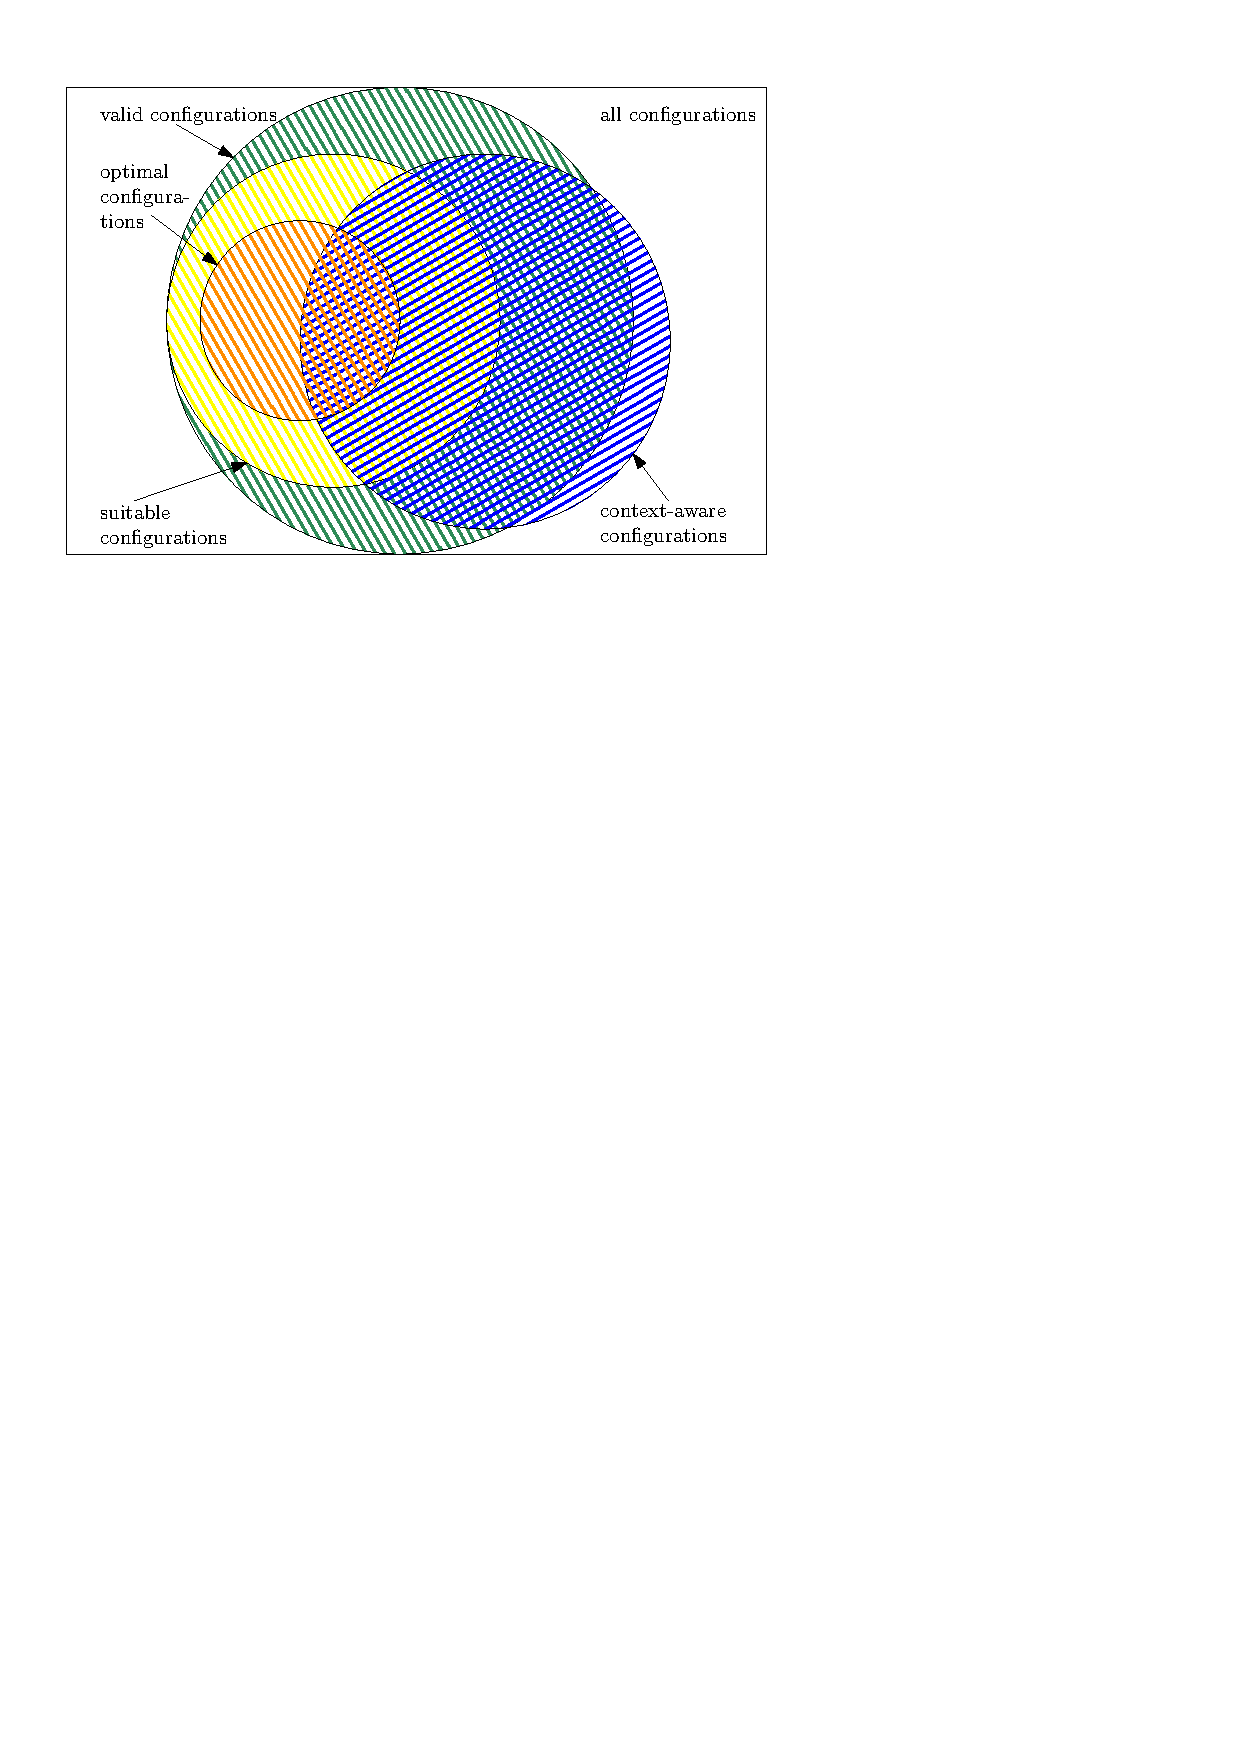
\includegraphics{configurations}
\end{frame}

\begin{frame}
	\frametitle{Viewpoints}
	\begin{description}
	\item[Sensors:] derive context from information sources of the system.
	Adding new context sensors increases the context available in a system.
	\ExecuteMetaData[../book/background.tex]{context-viewpoints}
	\end{description}
\end{frame}

\begin{frame}
	\frametitle{Cascading (Recapitulation)}
	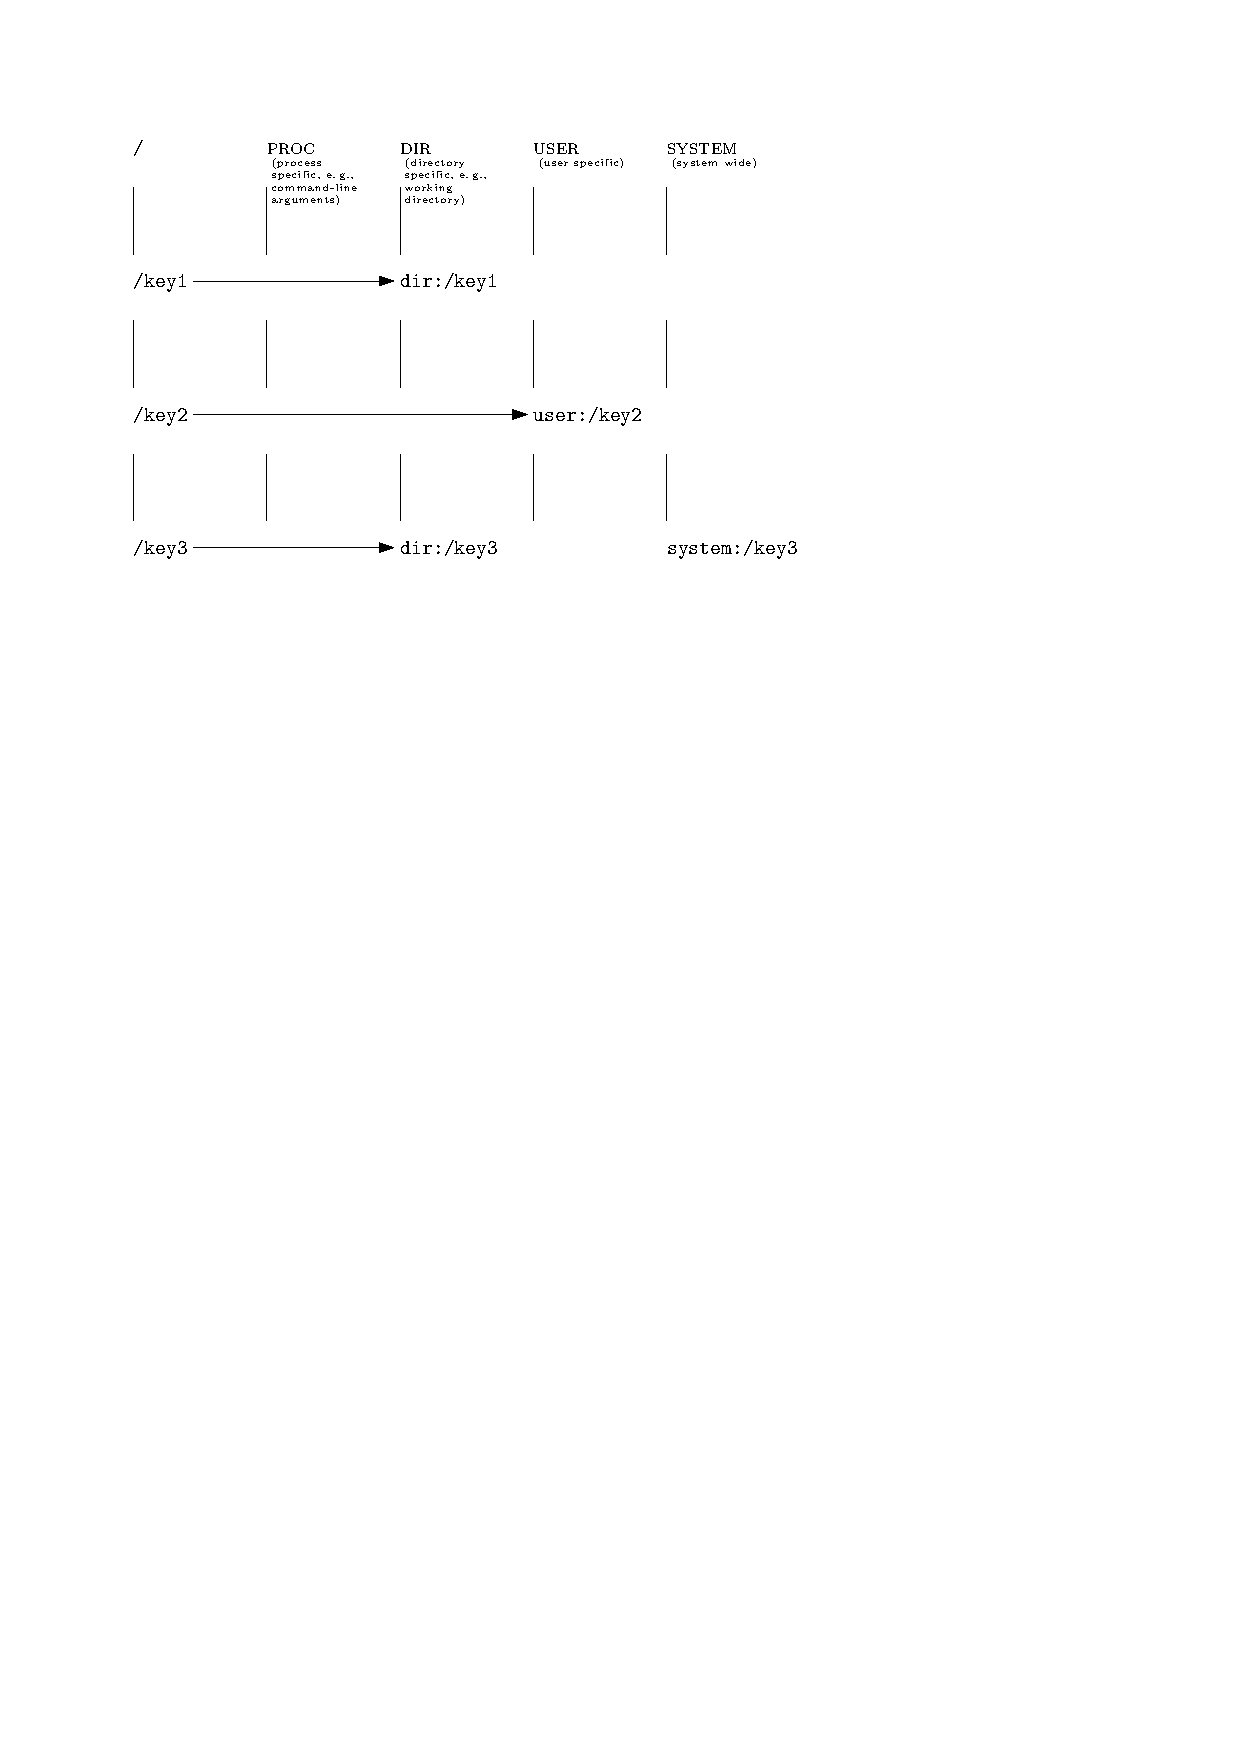
\includegraphics{cascading}
\end{frame}

\begin{frame}[fragile]
	\frametitle{Context-aware Lookup}

	\begin{itemize}
	\item
	Determine threads from CPUs:

	\begin{code}[gobble=4]
	[env/layer/cpu]
	  type:=long
	[slapd/threads/listener]
	  context:=/slapd/threads/%cpu%/listener
	\end{code}

	\item
	Determine vibration from sensors:

	\begin{code}[gobble=4]
	[phone/call/vibration]
	  type:=boolean
	  context:=/phone/call/%inpocket%/vibration
	\end{code}

	\item
	Determine proxy settings from network:

	\begin{code}[gobble=4]
	[env/override/http_proxy]
	  context:=/http_proxy/%interface%/%network%
	\end{code}
	\end{itemize}
\end{frame}




%%%%%%%%%%%%%%%%%%%%%%%%%%%%%%%%%%%%%%%%%% 
\section{Meeting}

%TODO: more didactics (team work, ..)


%%%%%%%%%%%%%%%%%%%%%%%%%%%%%%%%%%%%%%%%%% 
\nocite{raab2017introducing}

\appendix

\begin{frame}[allowframebreaks]
	\bibliographystyle{plainnat}
	\bibliography{../shared/elektra.bib}
\end{frame}

\end{document}

